\chapter{Map}

\clearpage
\section{Scans on map}

A mobile phone can carry out power measurements on the frequency currently in use, on serving and neighbour cells frequencies. The system may have multiple measurements in each location for serving cell and neighbor cells. Depending on the settings you make in the system, you can see the average, maximum or minimum of results for each location.

%===========================
% Technology on Map
\AddMapAllLeg{Map-Serving Cell-Technology---}{Technology parameter for Serving cell}

%%
%======== Power, Serving Cell, 2G
\AddMapAllLeg{Map-Scan-Serving-SigPow-2G-Avg}%
{Average Received signal power (\textit{RxLev}) for 2G serving cell}

\AddMapAllLeg{Map-Scan-Serving-SigPow-2G-Min}%
{Minimum Received signal power (\textit{RxLev}) for 2G serving cell}

\AddMapAllLeg{Map-Scan-Serving-SigPow-2G-Max}%
{Maximum Received signal power (\textit{RxLev}) for 2G serving cell}


%======== Power, Neighbor Cell, 2G
\AddMapAllLeg{Map-Scan-Neighbor-SigPow-2G-Avg}%
{Average Received signal power (\textit{RxLev}) for 2G neighbor cell}

\AddMapAllLeg{Map-Scan-Neighbor-SigPow-2G-Min}%
{Minimum Received signal power (\textit{RxLev}) for 2G neighbor cell}

\AddMapAllLeg{Map-Scan-Neighbor-SigPow-2G-Max}%
{Maximum Received signal power (\textit{RxLev}) for 2G neighbor cell}


%======== Power, Serving and Neighbor Cell, 2G
\AddMapAllLeg{Map-Scan-Serving,Neighbor-SigPow-2G-Avg}%
{Average Received signal power (\textit{RxLev}) for 2G serving and neighbor cell}

\AddMapAllLeg{Map-Scan-Serving,Neighbor-SigPow-2G-Min}%
{Minimum Received signal power (\textit{RxLev}) for 2G serving and neighbor cell}

\AddMapAllLeg{Map-Scan-Serving,Neighbor-SigPow-2G-Max}%
{Maximum Received signal power (\textit{RxLev}) for 2G serving and neighbor cell}


%======== Power, Serving Cell, 3G
\AddMapAllLeg{Map-Scan-Serving-SigPow-3G-Avg}%
{Average Received Signal Code Power (\textit{RSCP}) for 3G serving cell}

\AddMapAllLeg{Map-Scan-Serving-SigPow-3G-Min}%
{Minimum Received Signal Code Power (\textit{RSCP}) for 3G serving cell}

\AddMapAllLeg{Map-Scan-Serving-SigPow-3G-Max}%
{Maximum Received Signal Code Power (\textit{RSCP}) for 3G serving cell}


%======== Quality, Serving Cell, 3G
\AddMapAllLeg{Map-Scan-Serving-SigQual-3G-Avg}%
{Average Signal Quality (\textit{Ec/N0}) for 3G serving cell}

\AddMapAllLeg{Map-Scan-Serving-SigQual-3G-Min}%
{Minimum Signal Quality (\textit{Ec/N0}) for 3G serving cell}

\AddMapAllLeg{Map-Scan-Serving-SigQual-3G-Max}%
{Maximum Signal Quality (\textit{Ec/N0}) for 3G serving cell}


%======== Power, Neighbor Cell, 3G
\AddMapAllLeg{Map-Scan-Neighbor-SigPow-3G-Avg}%
{Average Received Signal Code Power (\textit{RSCP}) for 3G neighbor cell}

\AddMapAllLeg{Map-Scan-Neighbor-SigPow-3G-Min}%
{Minimum Received Signal Code Power (\textit{RSCP}) for 3G neighbor cell}

\AddMapAllLeg{Map-Scan-Neighbor-SigPow-3G-Max}%
{Maximum Received Signal Code Power (\textit{RSCP}) for 3G neighbor cell}


%======== Quality, Neighbor Cell, 3G
\AddMapAllLeg{Map-Scan-Neighbor-SigQual-3G-Avg}%
{Average Signal Quality (\textit{Ec/N0}) for 3G neighbor cell}

\AddMapAllLeg{Map-Scan-Neighbor-SigQual-3G-Min}%
{Minimum Signal Quality (\textit{Ec/N0}) for 3G neighbor cell}

\AddMapAllLeg{Map-Scan-Neighbor-SigQual-3G-Max}%
{Maximum Signal Quality (\textit{Ec/N0}) for 3G neighbor cell}


%======== Power, Serving and Neighbor Cell, 3G
\AddMapAllLeg{Map-Scan-Serving,Neighbor-SigPow-3G-Avg}%
{Average Received Signal Code Power (\textit{RSCP}) for 3G serving and neighbor cell}

\AddMapAllLeg{Map-Scan-Serving,Neighbor-SigPow-3G-Min}%
{Minimum Received Signal Code Power (\textit{RSCP}) for 3G serving and neighbor cell}

\AddMapAllLeg{Map-Scan-Serving,Neighbor-SigPow-3G-Max}%
{Maximum Received Signal Code Power (\textit{RSCP}) for 3G serving and neighbor cell}


%======== Quality, Serving and Neighbor Cell, 3G
\AddMapAllLeg{Map-Scan-Serving,Neighbor-SigQual-3G-Avg}%
{Average Signal Quality (\textit{Ec/N0}) for 3G serving and neighbor cell}

\AddMapAllLeg{Map-Scan-Serving,Neighbor-SigQual-3G-Min}%
{Minimum Signal Quality (\textit{Ec/N0}) for 3G serving and neighbor cell}

\AddMapAllLeg{Map-Scan-Serving,Neighbor-SigQual-3G-Max}%
{Maximum Signal Quality (\textit{Ec/N0}) for 3G serving and neighbor cell}


%======== Power, Serving Cell, 4G
\AddMapAllLeg{Map-Scan-Serving-SigPow-4G-Avg}%
{Average Reference Signals Received Power (\textit{RSRP}) for 4G serving cell}

\clearpage
\vfill
\begin{figure}
	\centering
	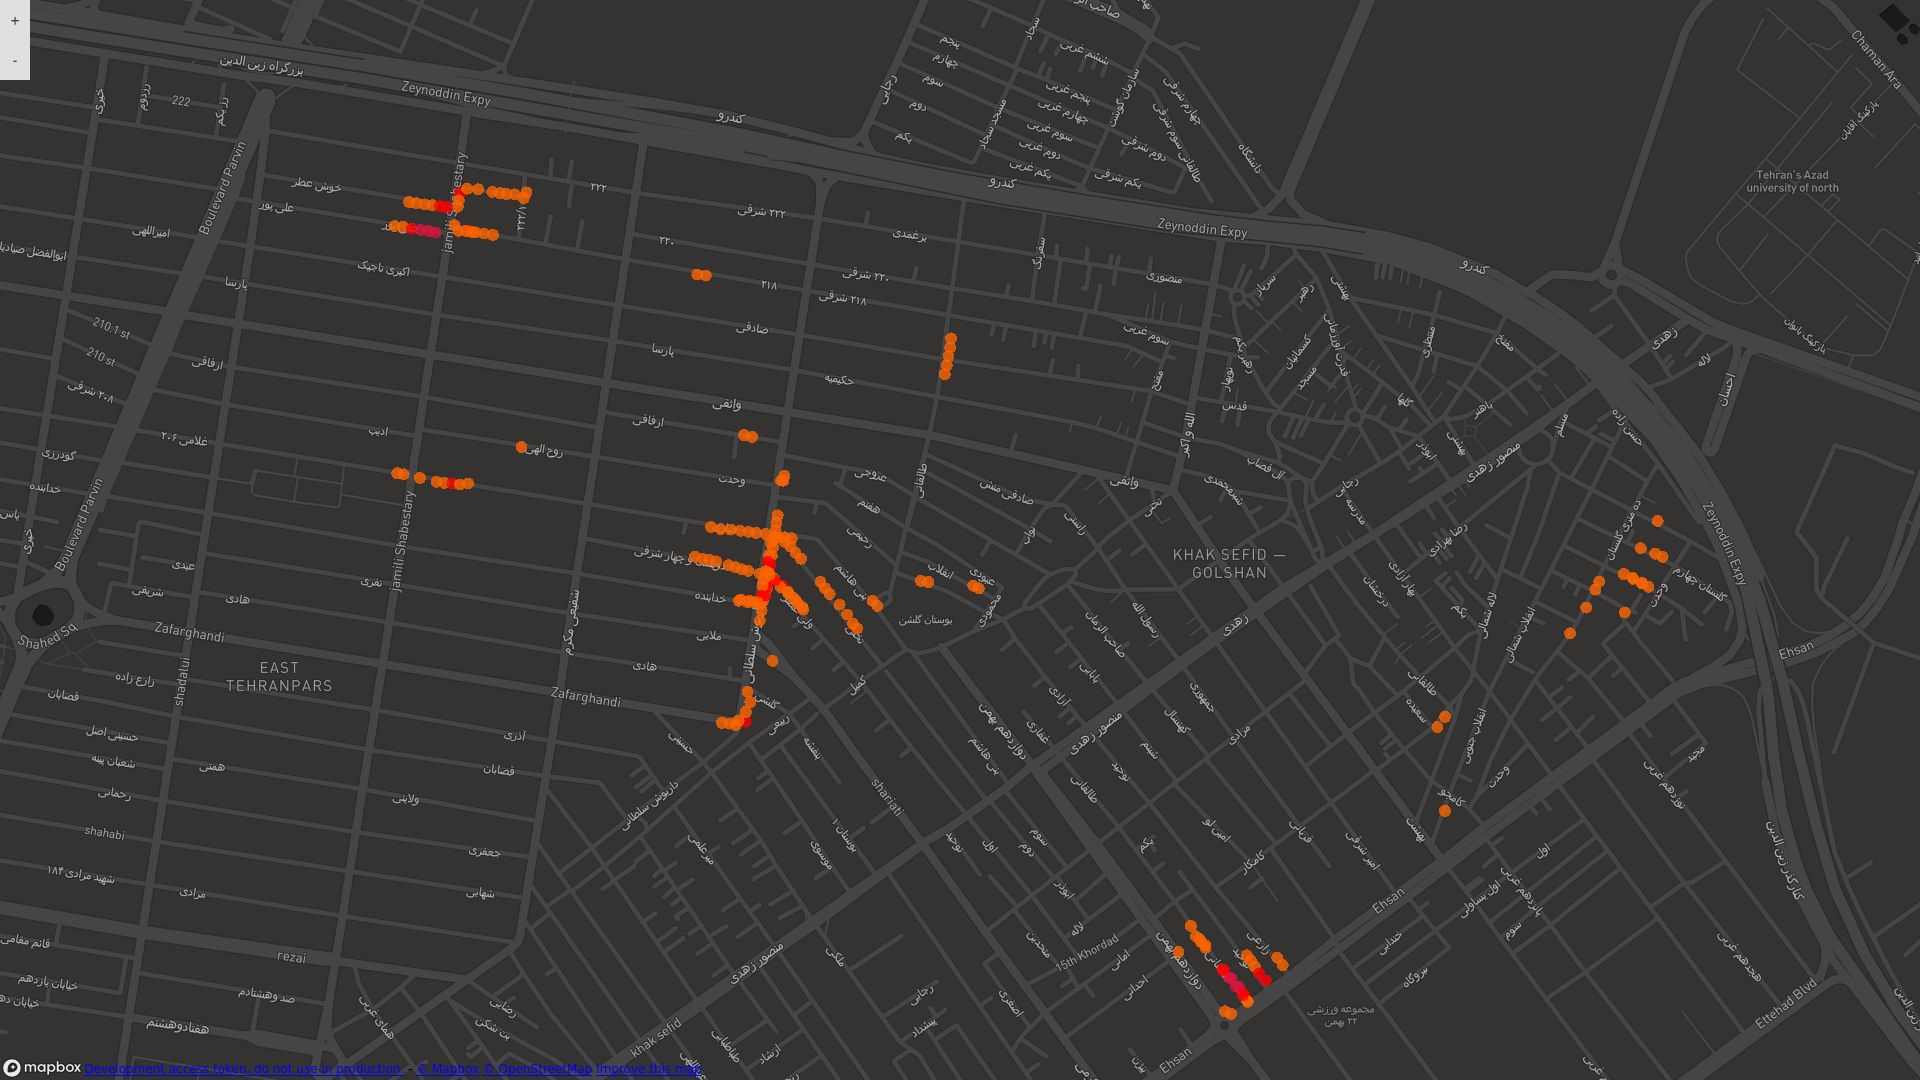
\includegraphics[width=\linewidth]{extraPic/BadRSRP}
	\caption{Just show RSRP less than \textit{Very Poor}}
	\label{fig:badrsrp}
\end{figure}
\vfill

\AddMapAllLeg{Map-Scan-Serving-SigPow-4G-Min}%
{Minimum Reference Signals Received Power (\textit{RSRP}) for 4G serving cell}

\AddMapAllLeg{Map-Scan-Serving-SigPow-4G-Max}%
{Maximum Reference Signals Received Power (\textit{RSRP}) for 4G serving cell}


%======== Quality, Serving Cell, 4G
\AddMapAllLeg{Map-Scan-Serving-SigQual-4G-Avg}%
{Average Reference Signal Received Quality (RSRQ) for 4G serving cell}

\clearpage
\vfill
\begin{figure}
	\centering
	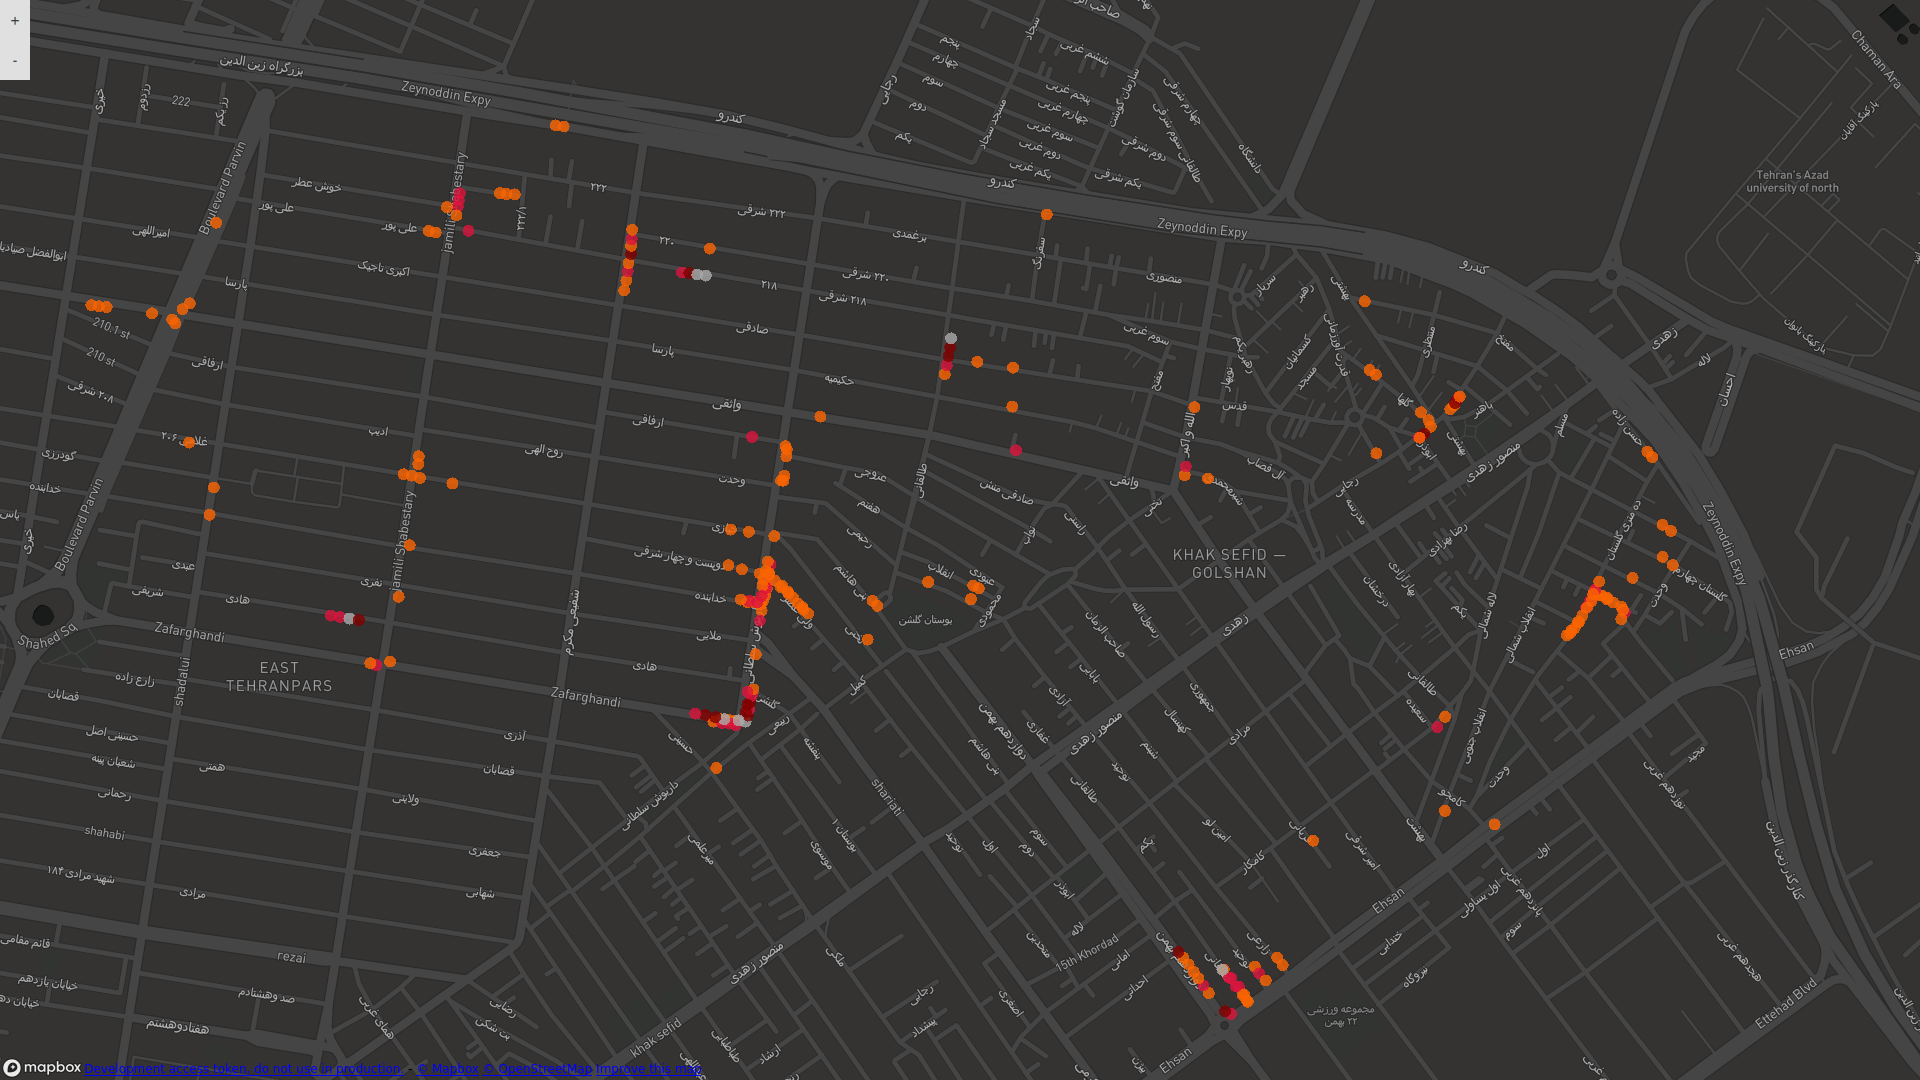
\includegraphics[width=\linewidth]{extraPic/BadRSRQ}
	\caption{Just show RSRQ less than \textit{Very Poor}}
	\label{fig:badrsrq}
\end{figure}
\vfill

\AddMapAllLeg{Map-Scan-Serving-SigQual-4G-Min}%
{Minimum Reference Signal Received Quality (RSRQ) for 4G serving cell}

\AddMapAllLeg{Map-Scan-Serving-SigQual-4G-Max}%
{Maximum Reference Signal Received Quality (RSRQ) for 4G serving cell}


\AddMapAllLeg{Map-Scan-Serving-SigSINR-4G-Min}%
{Minimum Signal to Interference plus Noise Ratio (SINR) for 4G serving cell}

\AddMapAllLeg{Map-Scan-Serving-SigSINR-4G-Max}%
{Maximum Signal to Interference plus Noise Ratio (SINR) for 4G serving cell}

%======== RSSI, Serving Cell, 4G
\AddMapAllLeg{Map-Scan-Serving-SigRSSI-4G-Avg}%
{Average Received Signal Strength Indication (RSSI) for 4G serving cell}

\AddMapAllLeg{Map-Scan-Serving-SigRSSI-4G-Min}%
{Minimum Received Signal Strength Indication (RSSI) for 4G serving cell}

\AddMapAllLeg{Map-Scan-Serving-SigRSSI-4G-Max}%
{Maximum Received Signal Strength Indication (RSSI) for 4G serving cell}


%======== Power, Neighbor Cell, 4G
\AddMapAllLeg{Map-Scan-Neighbor-SigPow-4G-Avg}%
{Average Reference Signals Received Power (\textit{RSRP}) for 4G neighbor cell}

\AddMapAllLeg{Map-Scan-Neighbor-SigPow-4G-Min}%
{Minimum Reference Signals Received Power (\textit{RSRP}) for 4G neighbor cell}

\AddMapAllLeg{Map-Scan-Neighbor-SigPow-4G-Max}%
{Maximum Reference Signals Received Power (\textit{RSRP}) for 4G neighbor cell}


%======== Quality, Neighbor Cell, 4G
\AddMapAllLeg{Map-Scan-Neighbor-SigQual-4G-Avg}%
{Average Reference Signal Received Quality (RSRQ) for 4G neighbor cell}

\AddMapAllLeg{Map-Scan-Neighbor-SigQual-4G-Min}%
{Minimum Reference Signal Received Quality (RSRQ) for 4G neighbor cell}

\AddMapAllLeg{Map-Scan-Neighbor-SigQual-4G-Max}%
{Maximum Reference Signal Received Quality (RSRQ) for 4G neighbor cell}


%======== Power, Serving and Neighbor Cell, 4G
\AddMapAllLeg{Map-Scan-Serving,Neighbor-SigPow-4G-Avg}%
{Average Reference Signals Received Power (\textit{RSRP}) for 4G serving and neighbor cell}

\AddMapAllLeg{Map-Scan-Serving,Neighbor-SigPow-4G-Min}%
{Minimum Reference Signals Received Power (\textit{RSRP}) for 4G serving and neighbor cell}

\AddMapAllLeg{Map-Scan-Serving,Neighbor-SigPow-4G-Max}%
{Maximum Reference Signals Received Power (\textit{RSRP}) for 4G serving and neighbor cell}


%======== Quality, Serving and Neighbor Cell, 4G
\AddMapAllLeg{Map-Scan-Serving,Neighbor-SigQual-4G-Avg}%
{Average Reference Signal Received Quality (RSRQ) for 4G serving and neighbor cell}

\AddMapAllLeg{Map-Scan-Serving,Neighbor-SigQual-4G-Min}%
{Minimum Reference Signal Received Quality (RSRQ) for 4G serving and neighbor cell}

\AddMapAllLeg{Map-Scan-Serving,Neighbor-SigQual-4G-Max}%
{Maximum Reference Signal Received Quality (RSRQ) for 4G serving and neighbor cell}


%%===========================
% 5G Serving Cell Power
\IfFileExists{./pic/Map-Scan-5G-Serving,Power.png}{%
\begin{figure}[H]\centering
\begin{tikzpicture}
\node [](P){\includegraphics[width=\textwidth,height=\textheight,keepaspectratio]{./pic/Map-Scan-5G-Serving,Power}};
\node at(P.south west)[above right,shape=rectangle,fill=white]{\input{./legend/Map-Scan-5G-Serving,Power}};
\end{tikzpicture}
\caption{Reference Signals Received Power (\textit{RSRP}) for 5G serving cell}
\end{figure}
}{}


%===========================
% 5G Serving Cell Quality
\IfFileExists{./pic/Map-Scan-5G-Serving,Quality.png}{%
\begin{figure}[H]\centering
\begin{tikzpicture}
\node [](P){\includegraphics[width=\textwidth,height=\textheight,keepaspectratio]{./pic/Map-Scan-5G-Serving,Quality}};
\node at(P.south west)[above right,shape=rectangle,fill=white]{\input{./legend/Map-Scan-5G-Serving,Quality}};
\end{tikzpicture}
\caption{Reference Signal Received Quality (RSRQ) for 5G serving cell}
\end{figure}
}{}


%===========================
% 5G Neighbor Cell Power
\IfFileExists{./pic/Map-Scan-5G-Neighbor,Power.png}{%
\begin{figure}[H]\centering
\begin{tikzpicture}
\node [](P){\includegraphics[width=\textwidth,height=\textheight,keepaspectratio]{./pic/Map-Scan-5G-Neighbor,Power}};
\node at(P.south west)[above right,shape=rectangle,fill=white]{\input{./legend/Map-Scan-5G-Neighbor,Power}};
\end{tikzpicture}
\caption{Reference Signals Received Power (\textit{RSRP}) for 5G neighbor cells}
\end{figure}
}{}


%===========================
% 5G Neighbor Cell Quality
\IfFileExists{./pic/Map-Scan-5G-Neighbor,Quality.png}{%
\begin{figure}[H]\centering
\begin{tikzpicture}
\node [](P){\includegraphics[width=\textwidth,height=\textheight,keepaspectratio]{./pic/Map-Scan-5G-Neighbor,Quality}};
\node at(P.south west)[above right,shape=rectangle,fill=white]{\input{./legend/Map-Scan-5G-Neighbor,Quality}};
\end{tikzpicture}
\caption{Reference Signal Received Quality (RSRQ) for 5G neighbor cells}
\end{figure}
}{}


%===========================
% 5G Serving and Neighbor Cells Power
\IfFileExists{./pic/Map-Scan-5G-Serving+Neighbor,Power.png}{%
\begin{figure}[H]\centering
\begin{tikzpicture}
\node [](P){\includegraphics[width=\textwidth,height=\textheight,keepaspectratio]{./pic/Map-Scan-5G-Serving+Neighbor,Power}};
\node at(P.south west)[above right,shape=rectangle,fill=white]{\input{./legend/Map-Scan-5G-Serving+Neighbor,Power}};
\end{tikzpicture}
\caption{Reference Signals Received Power (\textit{RSRP}) for 5G serving and neighbor cells}
\end{figure}
}{}


%===========================
% 5G Serving and Neighbor Cells Quality
\IfFileExists{./pic/Map-Scan-5G-Serving+Neighbor,Quality.png}{%
\begin{figure}[H]\centering
\begin{tikzpicture}
\node [](P){\includegraphics[width=\textwidth,height=\textheight,keepaspectratio]{./pic/Map-Scan-5G-Serving+Neighbor,Quality}};
\node at(P.south west)[above right,shape=rectangle,fill=white]{\input{./legend/Map-Scan-5G-Serving+Neighbor,Quality}};
\end{tikzpicture}
\caption{Reference Signal Received Quality (RSRQ) for 5G serving and neighbor cells}
\end{figure}
}{}


%======== Power, Serving Cell, 2G
\AddMapAllLegInfoOut{Map-Scan-Serving-SigPow-2G,3G-Avg}%
{Average \textit{RxLev} in 2G and \textit{RSCP} in 3G for serving cell}

\AddMapAllLegInfoOut{Map-Scan-Serving-SigPow-2G,3G-Min}%
{Minimum \textit{RxLev} in 2G and \textit{RSCP} in 3G  for serving cell}

\AddMapAllLegInfoOut{Map-Scan-Serving-SigPow-2G,3G-Max}%
{Maximum \textit{RxLev} in 2G and \textit{RSCP} in 3G for serving cell}


%======== Power, Neighbor Cell, 2G
\AddMapAllLegInfoOut{Map-Scan-Neighbor-SigPow-2G,3G-Avg}%
{Average \textit{RxLev} in 2G and \textit{RSCP} in 3G for neighbor cell}

\AddMapAllLegInfoOut{Map-Scan-Neighbor-SigPow-2G,3G-Min}%
{Minimum \textit{RxLev} in 2G and \textit{RSCP} in 3G  for neighbor cell}

\AddMapAllLegInfoOut{Map-Scan-Neighbor-SigPow-2G,3G-Max}%
{Maximum \textit{RxLev} in 2G and \textit{RSCP} in 3G for neighbor cell}


%======== Power, Serving and Neighbor Cell, 2G
\AddMapAllLegInfoOut{Map-Scan-Serving,Neighbor-SigPow-2G,3G-Avg}%
{Average \textit{RxLev} in 2G and \textit{RSCP} in 3G for serving and neighbor cell}

\AddMapAllLegInfoOut{Map-Scan-Serving,Neighbor-SigPow-2G,3G-Min}%
{Minimum \textit{RxLev} in 2G and \textit{RSCP} in 3G for serving and neighbor cell}

\AddMapAllLegInfoOut{Map-Scan-Serving,Neighbor-SigPow-2G,3G-Max}%
{Maximum \textit{RxLev} in 2G and \textit{RSCP} in 3G for serving and neighbor cell}


%======== Power, Serving Cell, 2G
\AddMapAllLegInfoOut{Map-Scan-Serving-SigPow-2G,4G-Avg}%
{Average \textit{RxLev} in 2G and \textit{RSRP} in 4G for serving cell}

\AddMapAllLegInfoOut{Map-Scan-Serving-SigPow-2G,4G-Min}%
{Minimum \textit{RxLev} in 2G and \textit{RSRP} in 4G  for serving cell}

\AddMapAllLegInfoOut{Map-Scan-Serving-SigPow-2G,4G-Max}%
{Maximum \textit{RxLev} in 2G and \textit{RSRP} in 4G for serving cell}


%======== Power, Neighbor Cell, 2G
\AddMapAllLegInfoOut{Map-Scan-Neighbor-SigPow-2G,4G-Avg}%
{Average \textit{RxLev} in 2G and \textit{RSRP} in 4G for neighbor cell}

\AddMapAllLegInfoOut{Map-Scan-Neighbor-SigPow-2G,4G-Min}%
{Minimum \textit{RxLev} in 2G and \textit{RSRP} in 4G  for neighbor cell}

\AddMapAllLegInfoOut{Map-Scan-Neighbor-SigPow-2G,4G-Max}%
{Maximum \textit{RxLev} in 2G and \textit{RSRP} in 4G for neighbor cell}


%======== Power, Serving and Neighbor Cell, 2G
\AddMapAllLegInfoOut{Map-Scan-Serving,Neighbor-SigPow-2G,4G-Avg}%
{Average \textit{RxLev} in 2G and \textit{RSRP} in 4G for serving and neighbor cell}

\AddMapAllLegInfoOut{Map-Scan-Serving,Neighbor-SigPow-2G,4G-Min}%
{Minimum \textit{RxLev} in 2G and \textit{RSRP} in 4G for serving and neighbor cell}

\AddMapAllLegInfoOut{Map-Scan-Serving,Neighbor-SigPow-2G,4G-Max}%
{Maximum \textit{RxLev} in 2G and \textit{RSRP} in 4G for serving and neighbor cell}


%======== Power, Serving Cell, 3G
\AddMapAllLegInfoOut{Map-Scan-Serving-SigPow-3G,4G-Avg}%
{Average \textit{RSCP} in 3G and \textit{RSRP} in 4G for serving cell}

\AddMapAllLegInfoOut{Map-Scan-Serving-SigPow-3G,4G-Min}%
{Minimum \textit{RSCP} in 3G and \textit{RSRP} in 4G  for serving cell}

\AddMapAllLegInfoOut{Map-Scan-Serving-SigPow-3G,4G-Max}%
{Maximum \textit{RSCP} in 3G and \textit{RSRP} in 4G for serving cell}


%======== Power, Neighbor Cell, 3G
\AddMapAllLegInfoOut{Map-Scan-Neighbor-SigPow-3G,4G-Avg}%
{Average \textit{RSCP} in 3G and \textit{RSRP} in 4G for neighbor cell}

\AddMapAllLegInfoOut{Map-Scan-Neighbor-SigPow-3G,4G-Min}%
{Minimum \textit{RSCP} in 3G and \textit{RSRP} in 4G  for neighbor cell}

\AddMapAllLegInfoOut{Map-Scan-Neighbor-SigPow-3G,4G-Max}%
{Maximum \textit{RSCP} in 3G and \textit{RSRP} in 4G for neighbor cell}


%======== Power, Serving and Neighbor Cell, 3G
\AddMapAllLegInfoOut{Map-Scan-Serving,Neighbor-SigPow-3G,4G-Avg}%
{Average \textit{RSCP} in 3G and \textit{RSRP} in 4G for serving and neighbor cell}

\AddMapAllLegInfoOut{Map-Scan-Serving,Neighbor-SigPow-3G,4G-Min}%
{Minimum \textit{RSCP} in 3G and \textit{RSRP} in 4G for serving and neighbor cell}

\AddMapAllLegInfoOut{Map-Scan-Serving,Neighbor-SigPow-3G,4G-Max}%
{Maximum \textit{RSCP} in 3G and \textit{RSRP} in 4G for serving and neighbor cell}



%======== Quality, Serving Cell, 3G
\AddMapAllLegInfoOut{Map-Scan-Serving-Quality-3G,4G-Avg}%
{Average \textit{Ec/N0} in 3G and \textit{RSRQ} in 4G for serving cell}

\AddMapAllLegInfoOut{Map-Scan-Serving-Quality-3G,4G-Min}%
{Minimum \textit{Ec/N0} in 3G and \textit{RSRQ} in 4G  for serving cell}

\AddMapAllLegInfoOut{Map-Scan-Serving-Quality-3G,4G-Max}%
{Maximum \textit{Ec/N0} in 3G and \textit{RSRQ} in 4G for serving cell}


%======== Quality, Neighbor Cell, 3G
\AddMapAllLegInfoOut{Map-Scan-Neighbor-Quality-3G,4G-Avg}%
{Average \textit{Ec/N0} in 3G and \textit{RSRQ} in 4G for neighbor cell}

\AddMapAllLegInfoOut{Map-Scan-Neighbor-Quality-3G,4G-Min}%
{Minimum \textit{Ec/N0} in 3G and \textit{RSRQ} in 4G  for neighbor cell}

\AddMapAllLegInfoOut{Map-Scan-Neighbor-Quality-3G,4G-Max}%
{Maximum \textit{Ec/N0} in 3G and \textit{RSRQ} in 4G for neighbor cell}


%======== Quality, Serving and Neighbor Cell, 3G
\AddMapAllLegInfoOut{Map-Scan-Serving,Neighbor-Quality-3G,4G-Avg}%
{Average \textit{Ec/N0} in 3G and \textit{RSRQ} in 4G for serving and neighbor cell}

\AddMapAllLegInfoOut{Map-Scan-Serving,Neighbor-Quality-3G,4G-Min}%
{Minimum \textit{Ec/N0} in 3G and \textit{RSRQ} in 4G for serving and neighbor cell}

\AddMapAllLegInfoOut{Map-Scan-Serving,Neighbor-Quality-3G,4G-Max}%
{Maximum \textit{Ec/N0} in 3G and \textit{RSRQ} in 4G for serving and neighbor cell}



%======== Power, Serving Cell, 3G
\AddMapAllLegInfoOut{Map-Scan-Serving-SigPow-2G,3G,4G-Avg}%
{Average \textit{RxLev} in 2G, \textit{RSCP} in 3G and \textit{RSRP} in 4G for serving cell}

\AddMapAllLegInfoOut{Map-Scan-Serving-SigPow-2G,3G,4G-Min}%
{Minimum \textit{RxLev} in 2G, \textit{RSCP} in 3G and \textit{RSRP} in 4G  for serving cell}

\AddMapAllLegInfoOut{Map-Scan-Serving-SigPow-2G,3G,4G-Max}%
{Maximum \textit{RxLev} in 2G, \textit{RSCP} in 3G and \textit{RSRP} in 4G for serving cell}


%======== Power, Neighbor Cell, 3G
\AddMapAllLegInfoOut{Map-Scan-Neighbor-SigPow-2G,3G,4G-Avg}%
{Average \textit{RxLev} in 2G, \textit{RSCP} in 3G and \textit{RSRP} in 4G for neighbor cell}

\AddMapAllLegInfoOut{Map-Scan-Neighbor-SigPow-2G,3G,4G-Min}%
{Minimum \textit{RxLev} in 2G, \textit{RSCP} in 3G and \textit{RSRP} in 4G  for neighbor cell}

\AddMapAllLegInfoOut{Map-Scan-Neighbor-SigPow-2G,3G,4G-Max}%
{Maximum \textit{RxLev} in 2G, \textit{RSCP} in 3G and \textit{RSRP} in 4G for neighbor cell}


%======== Power, Serving and Neighbor Cell, 3G
\AddMapAllLegInfoOut{Map-Scan-Serving,Neighbor-SigPow-2G,3G,4G-Avg}%
{Average \textit{RxLev} in 2G, \textit{RSCP} in 3G and \textit{RSRP} in 4G for serving and neighbor cell}

\AddMapAllLegInfoOut{Map-Scan-Serving,Neighbor-SigPow-2G,3G,4G-Min}%
{Minimum \textit{RxLev} in 2G, \textit{RSCP} in 3G and \textit{RSRP} in 4G for serving and neighbor cell}

\AddMapAllLegInfoOut{Map-Scan-Serving,Neighbor-SigPow-2G,3G,4G-Max}%
{Maximum \textit{RxLev} in 2G, \textit{RSCP} in 3G and \textit{RSRP} in 4G for serving and neighbor cell}



%======== Quality, Serving Cell, 3G
\AddMapAllLegInfoOut{Map-Scan-Serving-SigQual-2G,3G,4G-Avg}%
{Average \textit{Ec/N0} in 3G and \textit{RSRQ} in 4G for serving cell}

\AddMapAllLegInfoOut{Map-Scan-Serving-SigQual-2G,3G,4G-Min}%
{Minimum \textit{Ec/N0} in 3G and \textit{RSRQ} in 4G  for serving cell}

\AddMapAllLegInfoOut{Map-Scan-Serving-SigQual-2G,3G,4G-Max}%
{Maximum \textit{Ec/N0} in 3G and \textit{RSRQ} in 4G for serving cell}


%======== Quality, Neighbor Cell, 3G
\AddMapAllLegInfoOut{Map-Scan-Neighbor-SigQual-2G,3G,4G-Avg}%
{Average \textit{Ec/N0} in 3G and \textit{RSRQ} in 4G for neighbor cell}

\AddMapAllLegInfoOut{Map-Scan-Neighbor-SigQual-2G,3G,4G-Min}%
{Minimum \textit{Ec/N0} in 3G and \textit{RSRQ} in 4G  for neighbor cell}

\AddMapAllLegInfoOut{Map-Scan-Neighbor-SigQual-2G,3G,4G-Max}%
{Maximum \textit{Ec/N0} in 3G and \textit{RSRQ} in 4G for neighbor cell}


%======== Quality, Serving and Neighbor Cell, 3G
\AddMapAllLegInfoOut{Map-Scan-Serving,Neighbor-SigQual-2G,3G,4G-Avg}%
{Average \textit{Ec/N0} in 3G and \textit{RSRQ} in 4G for serving and neighbor cell}

\AddMapAllLegInfoOut{Map-Scan-Serving,Neighbor-SigQual-2G,3G,4G-Min}%
{Minimum \textit{Ec/N0} in 3G and \textit{RSRQ} in 4G for serving and neighbor cell}

\AddMapAllLegInfoOut{Map-Scan-Serving,Neighbor-SigQual-2G,3G,4G-Max}%
{Maximum \textit{Ec/N0} in 3G and \textit{RSRQ} in 4G for serving and neighbor cell}





\clearpage
\section{Serving Cell on map}
~ % Point: Do not remove it
\vfill
\begin{figure}[H]
\centering
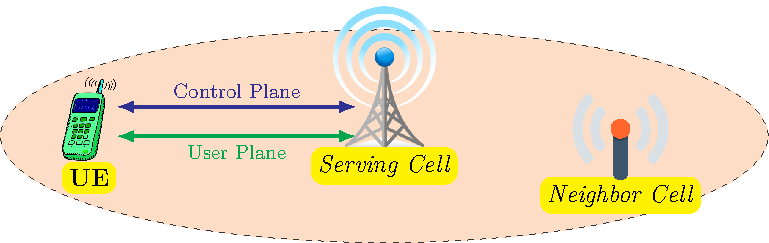
\includegraphics[width=.8\linewidth]{etc/UserPlaneControlPlane/mainFig}
\end{figure}
\vfill

\AddMapAllLeg{Map-Serving Cell-Technology---}{Technology parameter for Serving cell on map}
\AddPicNoLegend[0.8]{Serving Cells-Plot-----Tech.pdf}{Serving cell lifetime for each technology}

\AddPicLegOut{Serving Cells-Plot-----ARFCN-2G}{Serving cell lifetime for 2G}
\AddPicLegOut{Serving Cells-Plot-----ARFCN-3G}{Serving cell lifetime for 3G}
\AddPicLegOut{Serving Cells-Plot-----ARFCN-4G}{Serving cell lifetime for 4G}


\clearpage
\AddMapLegO{Map-Serving Cell-ARFCN---}{ARFCN parameter for Serving cell on map}

\AddPicLegOO{Map-Serving Cell-Code---}{Code parameter for Serving cell on map (Code in 2G=BSIC, 3G=PSC and 4G=PCI)}
\AddPicLegOO{Map-Serving Cell-ARFCN_Code---}{ARFCN/Code parameter for Serving cell on map (Code in 2G=BSIC, 3G=PSC and 4G=PCI)}
\AddPicLegOO{Map-Serving Cell-Cell Id---}{Cell Identity parameter for Serving cellon map}
\AddPicLegOO{Map-Serving Cell-PLMN Id---}{PLMN Identity parameter for Serving cell on map (Roaming)}
\AddPicLegOO{Map-Serving Cell-LAC---}{LAC/TAC parameter for Serving cell on map (2G and 3G=LAC, 4G=TAC)}
\clearpage
\vfill
\begin{figure}
	\centering
	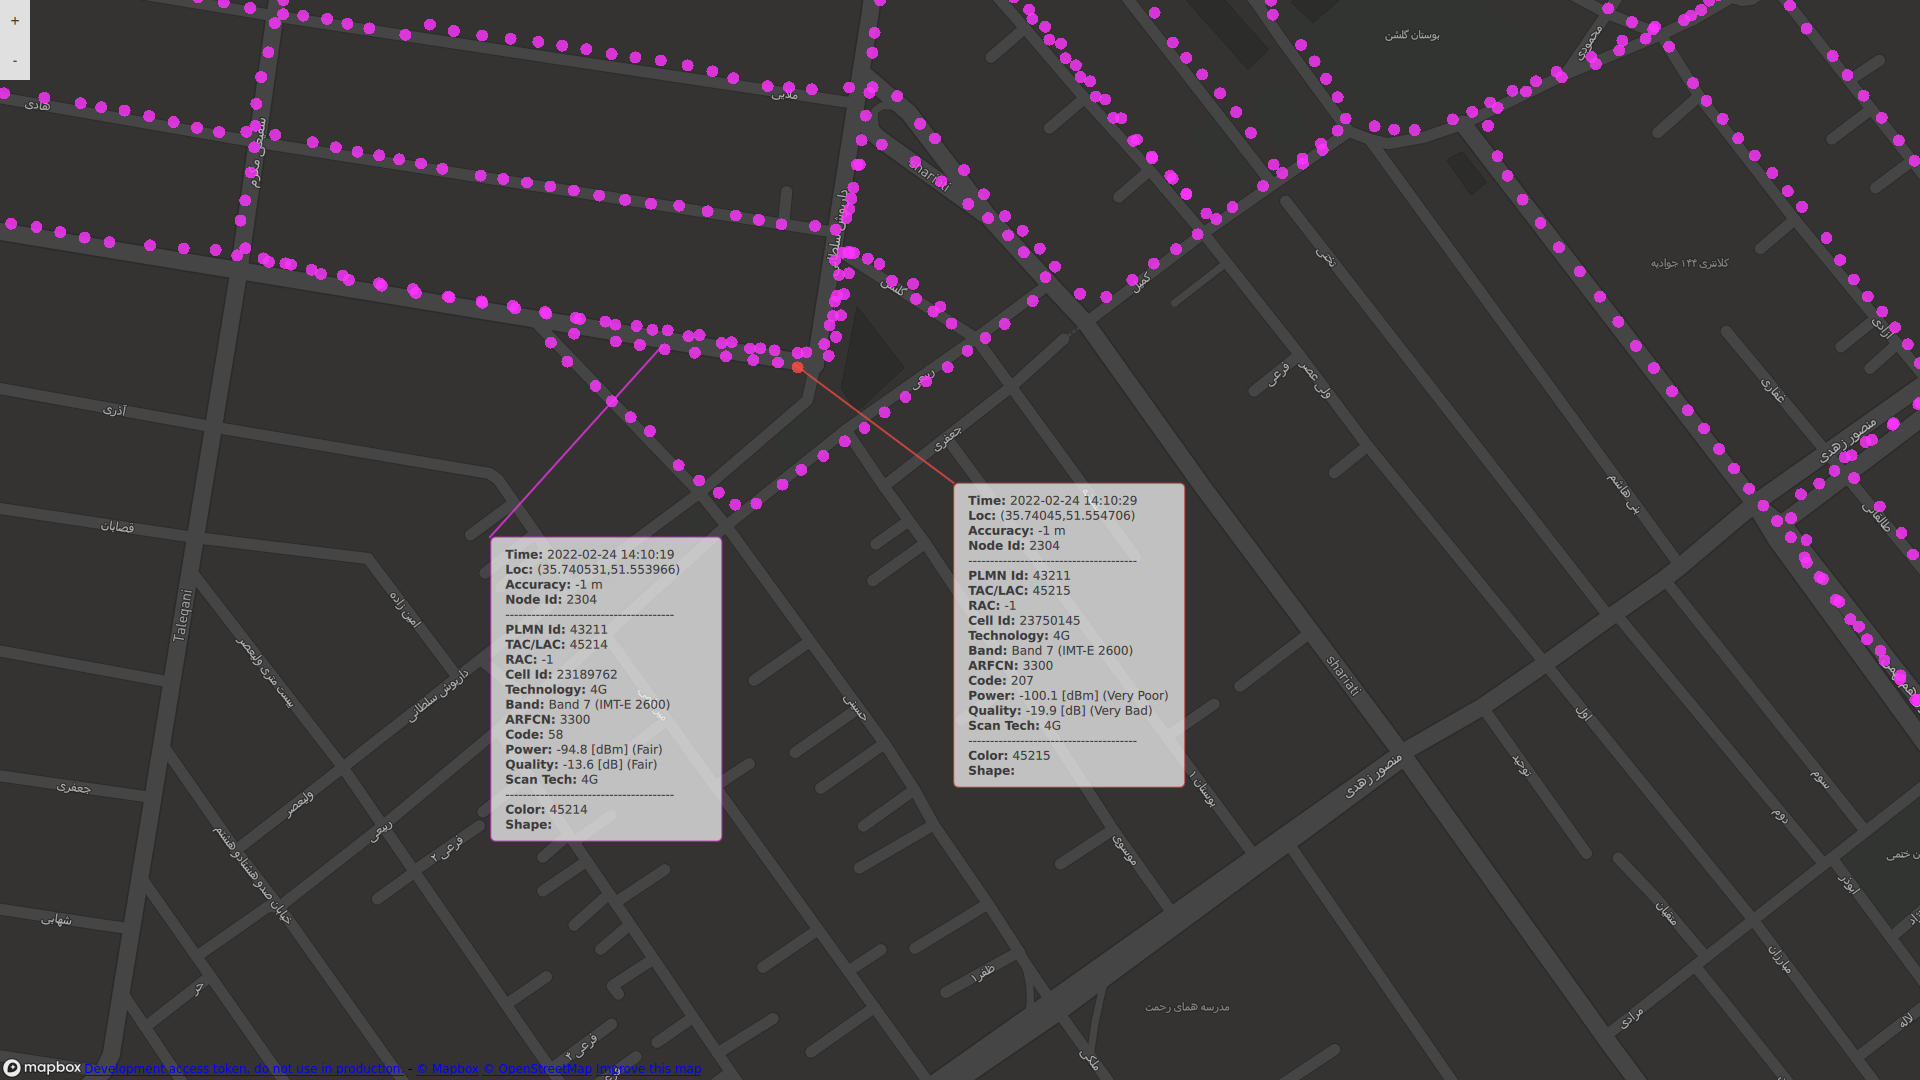
\includegraphics[width=\linewidth]{extraPic/AloneTAC}
	\caption{Alone TAC 45215}
	\label{fig:aloneTAC}
\end{figure}
\vfill

%\AddPicLegOO{Map-Serving Cell-RAC---}{RAC parameter for Serving cell on map}
